\documentclass[11pt,xcolor={dvipsnames},aspectratio=159,hyperref={pdftex,pdfpagemode=UseNone,hidelinks,pdfdisplaydoctitle=true},usepdftitle=false]{beamer}
\usepackage{presentation}[aspectratio=169]
\usepackage{math}
\usepackage{mathtools}
\usepackage{amsmath}
\usepackage{mleftright}

% Enter title of presentation PDF:
\hypersetup{pdftitle={Debt Sustainability}}
% Enter link to PDF file with figures:


\begin{document}
% Enter presentation title:
\title{Debt Sustainability}
\subtitle{Fiscal and Monetary Policy 2024}
% Enter presentation information:

% Enter presentation authors:
\author{Piotr Żoch}%
% Enter presentation location and date (optional; comment line if not needed):
\frame{\titlepage}

% Fill out content of presentation:
\begin{frame}{Plan}
    \begin{itemize}
    \item We review several approaches to debt sustainability analysis.
    \item Can the government service its current outstanding debt? Or will a fiscal consolidation be needed?
    \item Is the outstanding public debt and its projected path consistent with those of the government's revenues and expenditures?
   
    \end{itemize}
\end{frame}


\begin{frame}
    \heading{Classic Debt Sustainability Analysis}
\end{frame}

\begin{frame}{Debt to output ratio}

    \begin{itemize}
        \item The government static budget constraint is 
        \begin{align*}
            B_{t} = (1+r_{t})B_{t-1} + G_t - T_t.
        \end{align*}
        where $B_{t-1}$ is the \alb{market value} of all outstanding debt (all maturities), $G_t$ is nominal government spending (net of interest expenses), $T_t$ is nominal tax revenue, and $r_t$ is net nominal return on government debt.
        \item We abstract from money growth (we can treat money as a type of government debt).
        \item Note: it is often called ``flow budget constraint''. 
        \item Note: is it really a ``constraint''?
    \end{itemize}
\end{frame}
\begin{frame}{Debt to output ratio}

    \begin{itemize}
        \item Divide by \al{nominal} GDP $Y_t$ and rearrange  to get
        \begin{align*}
            \frac{B_{t}}{Y_t} = (1+r_{t})\frac{B_{t-1}}{Y_{t-1}}\frac{Y_{t-1}}{Y_t} + \frac{G_t}{Y_t} - \frac{T_t}{Y_t}.
        \end{align*}
        \item Define $$R_{t-j,t} \coloneq \prod_{k=1}^{j} \bp{1+r_{t-j+k}},$$ the cumulative return on debt from $t-j$ to $t$.
        \item Define $$X_{t-j,t} \coloneq \prod_{k=1}^{j} \frac{Y_{t-j+k}}{Y_{t-j+k-1}},$$ the cumulative gross growth rate of GDP from $t-j$ to $t$.
        
    \end{itemize}
\end{frame}

\begin{frame}{Debt to output ratio}

    \begin{itemize}
        \item For simplicity assume $B_0=0$.
        \item We can write the debt to output ratio as 
        \begin{align*}
            \frac{B_{t}}{Y_t} = \sum_{j=0}^t \frac{G_{t-j}-T_{t-j}}{Y_{t-j}} \frac{R_{t-j,t}}{X_{t-j,t}}
        \end{align*}
        \item Debt to output ratio today is determined by: 
        \begin{enumerate}
            \item The past primary deficits to GDP ratios;
            \item The past returns on debt;
            \item The past growth rates of (nominal) GDP.
        \end{enumerate}
        \item We can use the formula above to understand what determines the current debt to output ratio. 
    \end{itemize}
\end{frame}

\begin{frame}{Classic Debt Sustainability Analysis}
    \begin{itemize}
        \item A version of the formula is often used to assess \al{debt sustainability} -- "whether the government can service its debt".
        \item \alr{Warning}: this is about the future, not the present. The fact that people use the formula to assess the current situation is often a red flag!
        \item Classic debt sustainability analysis looks at the "long run".
        \end{itemize}
\end{frame}


\begin{frame}{Classic Debt Sustainability Analysis}
    \begin{itemize}
        \item Assume that the economy is in a steady state with a constant growth rate of GDP $X$, a constant rate of return $R$ and a constant primary deficit to GDP ratio.
        \item What is the debt to output ratio consistent with the above?
        \item If the observed current debt to output ratio is \al{below} this level, it is \al{sustainable}.
    \end{itemize}
\end{frame}

\begin{frame}{Classic Debt Sustainability Analysis}

    \begin{itemize}
        \item Classic debt sustainability analysis usually analyzes deterministic setups (or perfect foresight).
        \item In these setups, the appropriate $R$ is the \alb{risk-free rate}, $R^f$. 
        \item Assuming the above, the formula in the steady state becomes 
        \begin{align*}
            \frac{B}{Y} = \frac{G-T}{Y}\frac{X}{X-R^f}.
        \end{align*}
        \item For simplicity define $x\coloneqq X - 1$ and $r^f\coloneqq R^f - 1$ so we have         
        \begin{align*}
            \frac{B}{Y} = \frac{G-T}{Y}\frac{1+x}{x-r^f}.
        \end{align*}
        \item Hote: here $X$ and $R$ are one period rates (not cumulative). 
    \end{itemize}
\end{frame}

\begin{frame}{Classic Debt Sustainability Analysis}
    \begin{align*}
        \frac{B}{Y} = \frac{G-T}{Y}\frac{1+x}{x-r^f}
    \end{align*}
    \begin{itemize}
        \item Example: the Treaty of Maastricht set the limit of the debt to output ratio at 60\% and the deficit to output ratio at 3\%. What must be the growth rate of GDP and the risk-free rate for this to be sustainable?
        \end{itemize}
\end{frame}

\begin{frame}{Classic Debt Sustainability Analysis}
    \begin{align*}
        \frac{B}{Y} = \frac{G-T}{Y}\frac{1+x}{x-r^f}
    \end{align*}
    \begin{itemize}
        \item For $B\slash Y = 0.6$ and $G-T\slash Y = 0.03$ we have $\frac{0.6}{0.03} = 20$.
        \item We get $\frac{1+x}{x-r^f} = 20$.
        \item For small $x$ we have $x\approx r^f + 0.005$, so the economy has to grow at 0.5\% above the risk-free rate per year for the debt at the limit to be sustainable with the largest allowed deficit.
        \item If the actual growth rate is lower, the debt to output ratio will be larger, even if the deficit is at the limit.
    \end{itemize}
\end{frame}



\begin{frame}{Classic Debt Sustainability Analysis}
    \begin{align*}
        \frac{B}{Y} = \frac{G-T}{Y}\frac{1+x}{x-r^f}
    \end{align*}
    \begin{itemize}
        \item The key role of $x-r^f$.
        \item Depending on the sign of $x-r^f$ you require either surpluses or deficits to keep the debt to output ratio constant.
        \begin{itemize}
            \item If $x<r^f$ you need surpluses.
            \item If $x>r^f$ you can have deficits.
        \end{itemize}
        \item A big "r versus g" debate (we have $x$ instead of $g$). 
    \end{itemize}
\end{frame}

\begin{frame}{Classic Debt Sustainability Analysis}
    \begin{itemize}
        \item If $x>r^f$ it seems there is \al{no fiscal cost} to debt.
        \item Blanchard (2019) argues that $x>r^f$ is a norm, not an exception. 
        \item But what is $r^f$? How to measure it? Blanchard (2019) looks at the 1-year US Treasury bill rate, the 10-year US Treasury bond rate, adjusts for various maturities... 
        \item Note: it does not necessarily mean that it is \alb{optimal} to have deficits.
    \end{itemize}
\end{frame}

\begin{frame}{Rates in the US}
    \begin{figure}
        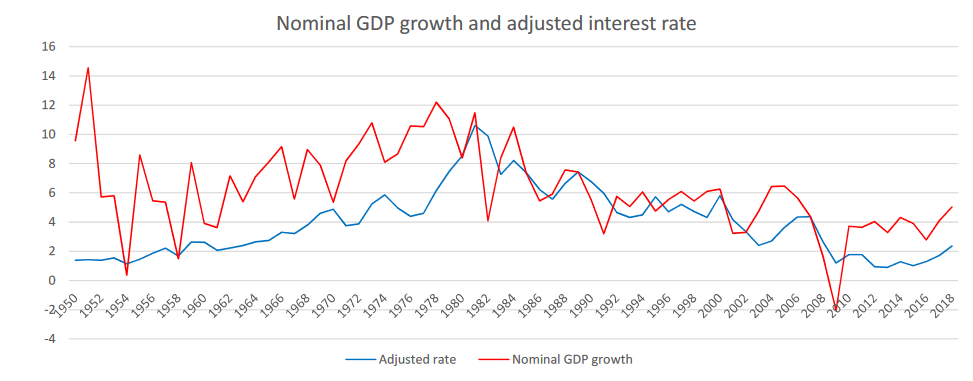
\includegraphics[width=1\textwidth]{blanchard_rg.png}
        \caption{Source: Blanchard (2019)}
    \end{figure}
   \end{frame}

\begin{frame}{Classic Debt Sustainability Analysis}
    \begin{itemize}
        \item It only \al{defines} what long-run debt
        is for a given long-run primary balance (or vice versa) \al{if} stationarity holds, or defines lower bounds on the
        short-run dynamics of the primary balance.
        \item It does not connect the outstanding initial debt of a
        particular period with the steady state.
        \item There might be multiple paths of debt that do not violate the \alb{intertemporal government budget constraint} (IGBC), some of them can even go to infinity (but slowly enough)!
        \item IGBC: the value of debt is equal to the present discounted value of future primary surpluses.
    \end{itemize}
\end{frame}

\begin{frame}
    \heading{Intertemporal Government Budget Constraint}
\end{frame}

\begin{frame}{IGBC}
    \begin{itemize}
        \item We used the government budget constraint by solving it \al{backward} (go back in time).
        \item We can also solve it \al{forward} -- the \alb{valuation approach}, the market value of government debt is determined by the discounted value of future government surpluses. 
        \item This idea is often used in finance (e.g., Campbell and Shiller 1988) - what determines stock prices?
        \item Allows us to think seriously about risk and asset pricing.
    \end{itemize}
\end{frame}

\begin{frame}{IGBC}
    \begin{itemize}
        \item Ignore risk for now and rewrite \begin{align*}             
            B_{t+1} = (1+r_{t+1})B_{t} + G_{t+1} - T_{t+1} \end{align*}
            as 
            \begin{align*}
                B_t =  \frac{1}{1+r_{t+1}}\bp{B_{t+1} - G_{t+1} + T_{t+1}}.
            \end{align*}
            \item Continue this process to get 
            \begin{align*}
                B_t = \sum_{j=1}^T \frac{1}{\prod_{k=1}^j (1+r_{t+k})} \bp{T_{t+j}-G_{t+j}} +\frac{1}{\prod_{k=1}^T (1+r_{t+k})}  B_{t+T}.
            \end{align*}
    \end{itemize}
\end{frame}

\begin{frame}{IGBC}
    \begin{itemize}
        \item Note: there is a term $\frac{1}{\prod_{k=1}^T (1+r_{t+k})}  B_{t+T}$. 
        \item If this term does not vanish as $T\to\infty$, there is a \al{bubble}.
        \item Imposing the no-Ponzi game condition ($\lim_{T\rightarrow \inf} \frac{1}{\prod_{k=1}^T (1+r_{t+k})}  B_{t+T} = 0$) on the above budget constraint, we get the IGBC: \begin{align*}
            B_t = \sum_{j=1}^\infty \frac{1}{\prod_{k=1}^j (1+r_{t+k})} \bp{T_{t+j}-G_{t+j}}.
        \end{align*}
        \item If the above is satisfied, we say that IGBC holds. 
        \end{itemize}
\end{frame}



\begin{frame}{IGBC}
    \begin{itemize}
        \item In a more general version IGBC is \begin{align*}
            B_t = \E_t \sum_{j=1}^\infty M_{t,t+j} \bp{T_{t+j}-G_{t+j}}
        \end{align*}
        \item We call $M_{t,t+j}$ the \alb{stochastic discount factor} (SDF). 
        \item It reflects how holders of government debt value discount future cash flows. 
        \item Generally it is a function of the state of the economy at time $t$ and $t+j$. Recall the first order condition for the household problem in the models we saw.
        \item We call the formula above the \alg{intertemporal government budget constraint} (IGBC).
        \end{itemize}
\end{frame}

\begin{frame}{Debt sustainability}
    \begin{itemize}
        \item We can say that debt is sustainable if and only if the IGBC holds.
        \item \al{Problem}: this condition is about the entire future. 
        \item \alb{Solution (?)}: use forecasts of future taxes and spending to compute the present value of future surpluses. Some early papers did this, but they used \alr{risk-free} rates.  
        \item Valid if one of these conditions holds: 
        \begin{enumerate}
            \item There is perfect foresight;
            \item Investors are risk-neutral;
            \item Primary surpluses do not covary with the SDF.
        \end{enumerate}
    \end{itemize}
\end{frame}


\begin{frame}{Bohn (1998)}
    \begin{itemize}
        \item Not even debt (or debt to GDP) going to infinity means that the IGBC does not hold, it has to go to infinity \al{slowly enough}.
        \item Bohn (1998): see if the government does something that guarantees the IGBC holds, investigate the \alb{fiscal reaction function}.
        \item Allows to sidestep the problem of forecasting future taxes and spending and choosing the correct discount rate.
        \item Sufficient condition: IGBC might also hold if it is violated, but if it is satisfied, IGBC holds for sure.
    \end{itemize}
\end{frame}

\begin{frame}{Bohn (1998)}
    \begin{itemize}
        \item Linear reaction function:
        \begin{align*}
            \frac{T_t - G_t}{Y_t} = \rho \frac{B_{t-1}}{Y_{t-1}} + Z_t + \epsilon_t
        \end{align*}
        \item The left hand side is \al{primary surplus}.
        \item $Z_t$ is a vector of exogenous variables that affect the primary surplus.
        \item Check if $\rho>0$ -- raise surplus if debt is high. 
        \item If $\rho>0$, then the \alb{IGBC holds} even if it is \alr{below} the interest rate (net of $x$).
    \end{itemize}
\end{frame}

\begin{frame}{Bohn (1998)}
    \begin{itemize}
        \item If $\rho>0$, the IGBC holds for \al{any} initial level of debt.
        \item This analysis works also for $r-x=0$ -- there was division by zero in the classic analysis.
        \item If $r-x>\rho>0$, debt explodes, but the IGBC \al{still} holds (under certain conditions: see Bohn 2007).
    \end{itemize}
\end{frame}

\begin{frame}{Bohn (1998)}
    \begin{itemize}
        \item Bohn (1998) estimates $\rho$ for the US in 1916-1995.
        \item He includes the level of temporary government spending and business cycle indicator in $Z_t$.
        \item He find a \al{positive} value of $\rho$, around 0.05 for the entire sample.
    \end{itemize}
\end{frame}

\begin{frame}{Bohn (1998)}
    \begin{figure}
        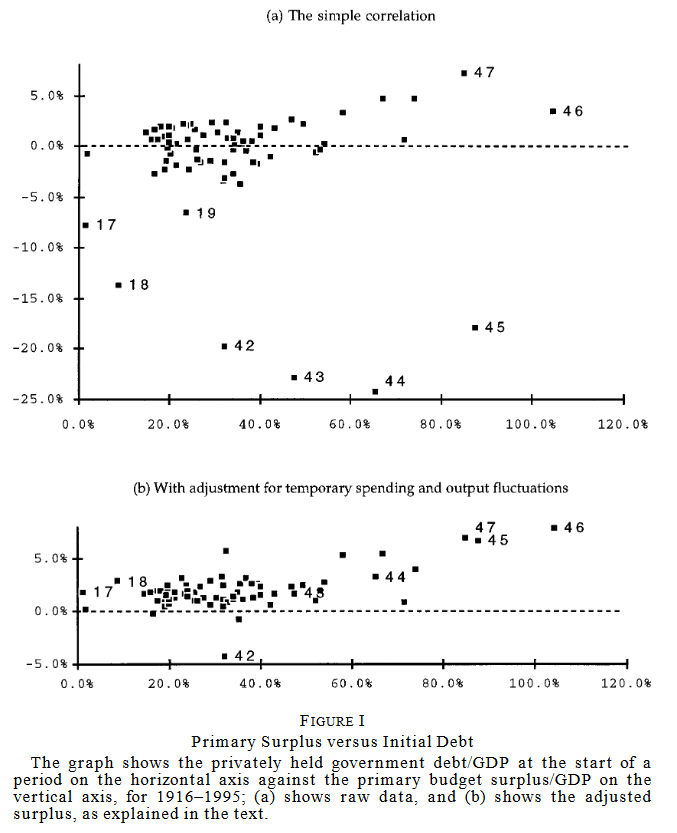
\includegraphics[width=0.5\textwidth]{bohn_1.png}
        \caption{Source: Bohn (1998)}
    \end{figure}
   \end{frame}

   \begin{frame}{Bohn (1998)}
    \begin{figure}
        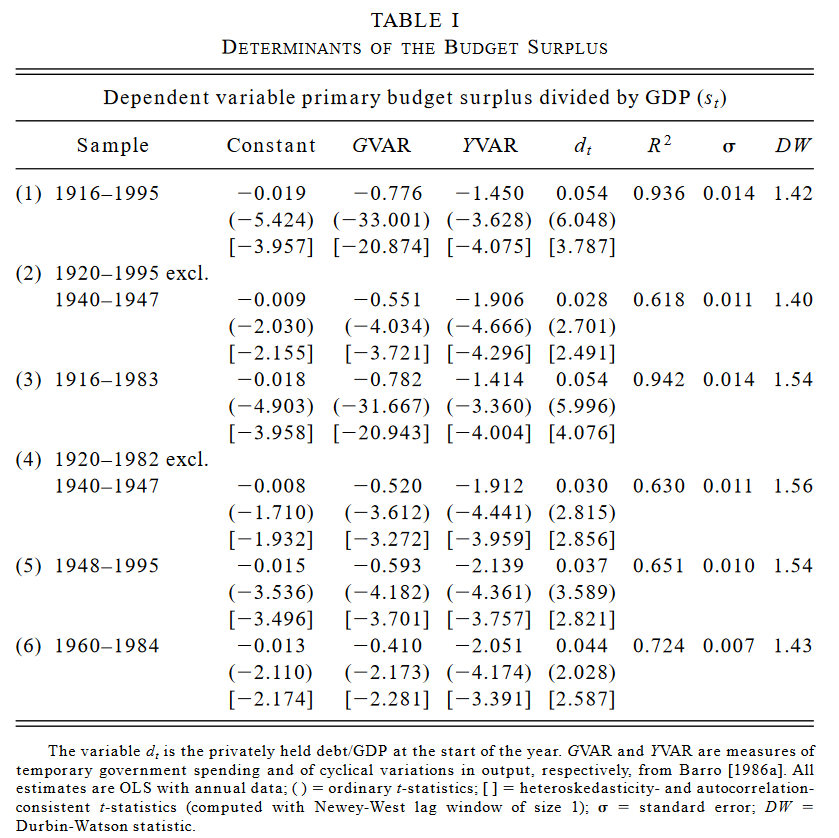
\includegraphics[width=0.6\textwidth]{bohn_2.png}
        \caption{Source: Bohn (1998)}
    \end{figure}
   \end{frame}

\begin{frame}{Fiscal reaction functions}
    \begin{itemize}
        \item Bohn (2008) extends the analysis to 1793-2003.
        \item He finds that $\rho>0.1$, more than twice as large as in the previous study.
        \item Mendoza and Ostry (2008) study fiscal reaction functions for a panel of multiple countries -- similar results.
        \item Ghosh et al. (2013) show that $\rho$ is much lower at high levels of debt. 
        \item D'Erasmo et al. (2016):
         \begin{enumerate}
            \item primary balance adjustment in the US after 2008 was \al{too large} to be explained by the fiscal reaction function;
            \item adjustment is \al{slower} than before (structural break);
            \item nevertheless, with the estimated $\rho$, the IGBC holds.
        \end{enumerate}
    \end{itemize}
\end{frame}

\begin{frame}{Fiscal reaction functions}
    \begin{itemize}
        \item Leeper (2017) warns against using surplus-debt regressions to assess debt sustainability.
        \item For the estimator of $\rho$ to be \alb{consistent}, we must have $$\E{\epsilon_t \mid \frac{B_{t-1}}{Y_{t-1}}} = 0.$$ \begin{enumerate}
            \item This means that shocks at $t-1$ that affect debt-output ratio in must not affect $\epsilon_t$.
            \item This means that the debt-output ratio cannot depend on the expectation of $\epsilon_t$.
        \end{enumerate}
        \item Since the value of debt depends on the expected value of future surpluses, this is a strong assumption: $\epsilon_t$ could be serially correlated.
    \end{itemize}
\end{frame}



\begin{frame}
    \heading{Valuation approach}
\end{frame}

\begin{frame}{Valuation approach}
    \begin{itemize}
        \item We go back to the budget constraint and solve it forward as 
        \begin{align*}
            B_t = \E_t \sum_{j=1}^T M_{t,t+j} \bp{T_{t+j}-G_{t+j}} + \E_t M_{t,t+T} B_{t+T}
        \end{align*}
        \item We obtained the standard IGBC if \begin{align*}
            \lim_{T\to\infty} \E_t M_{t,t+T} B_{t+T} = 0.
        \end{align*}
        \item The IGBC implies that a higher debt-to-output ratio today can be attributed to higher ex-
        pected future primary surpluses (cash flows) or lower expected future returns (discount rates).
        \item The counterpart of the Campbell-Shiller expression for the log of the price-to-dividend ratio in the stock market. 
    \end{itemize}
\end{frame}

\begin{frame}{Valuation approach}
    \begin{itemize}
        \item Cochrane (2011) shows that discount rate variation is
        the main driver of stock valuation ratios.
        \item Cochrane (2019): half of the variation in the debt-to-GDP ratio to variation in future primary surpluses and half to varying discount rates.
        \item Jiang et al. (2021) conclude \alr{no
        statistical evidence} of a discount rate or cash flow channel. 
        \item Fluctuation in the debt-to-GDP ratio at time $t$ predict fluctuations in the debt-to-GDP ratio at time $t+T$.
        \item Jiang et al. argue the differences result from small sample bias. 
    \end{itemize}
\end{frame}

\begin{frame}{Fiscal capacity}
    \begin{itemize}
        \item Jiang et al. in a series of recent papers propose a new approach to debt sustainability analysis.
        \item Suppose an investor buys the \al{entire} stock of government debt and participates in all new issuances. 
        \item How much would that investor be willing to pay for the debt?
        \item Cash flow is $\bc{T_t-G_t}$.
        \item Use tools from asset pricing to answer this question.
        \item The price will depend on the riskiness of the cash flows. 
    \end{itemize}
\end{frame}

\begin{frame}{Asset pricing basics}  
    \begin{itemize}
        \item Before we talk about Jiang et al., let's review some asset pricing basics. 
        \item The general idea dates back to Lucas (1978) who considers asset prices in a general equilibrium model.
        \item An asset is a claim on a stream of prospective payments.
        \item Consider an economy with $i=1,\dots,N$ assets.
        \item Each of this assets has an associated stream of real dividends $\bc{d_{i,t}}^\infty_{t=0}$. 
        \item Assume the representative investor maximizes $\E_0 \sum_{t=0}^\infty \beta^t u\of{c_t}$.
        \item Let $p_{i,t}$ be the price of asset $i$ at time $t$ (in goods).
    \end{itemize}
\end{frame}


\begin{frame}{Asset pricing basics}  
    \begin{itemize}
        \item For each asset the investor holds, the optimality condition is: 
\begin{align*}
        p_{i,t}  = \b \E_t \frac{u^\prime\of{c_{t+1}}}{u^\prime\of{c_t}} \bp{ p_{i,t+1} + d_{i,t+1}}.    
\end{align*}
\item This is the \al{consumption-based asset pricing equation}.
        \item We can slightly rearrange it as 
        \begin{align*}
            1  = \b \E_t \frac{u^\prime\of{c_{t+1}}}{u^\prime\of{c_t}} \frac{ p_{i,t+1} + d_{i,t+1}}{p_{i,t}}.    
    \end{align*}
    \item Here $R_{i,t,t+1}\coloneq \frac{ p_{i,t+1} + d_{i,t+1}}{p_{i,t}}$ is the (gross) rate of \alb{return} on asset $i$ from $t$ to $t+1$.
    \end{itemize}
\end{frame}

\begin{frame}{Asset pricing basics}  
    \begin{itemize}
        \item Define $M_{t,t+1}\coloneq \beta \frac{u^\prime\of{c_{t+1}}}{u^\prime\of{c_t}}$.
        \item We call it the \alb{stochastic discount factor} (SDF).
\item We can write the asset pricing equation for \al{each asset} as \begin{align*}
    1 = \E_t M_{t,t+1} R_{i,t,t+1}.
\end{align*}
\item The \alg{risk-free rate} $R^f_{t,t+1}$ satisfies \begin{align*} 
    1 = R^f_{t,t+1} \E_t M_{t,t+1}.
\end{align*}
        
\end{itemize}
\end{frame}


\begin{frame}{Asset pricing basics}  
    \begin{itemize}
        \item Sometimes you will see the asset pricing equation written as
        \begin{align*}
            v_{i,t} = \E_t M_{t,t+1} \frac{d_{i,t+1}}{d_t} \bp{1+v_{i,t+1}}.
        \end{align*}
        \item Here $v_{i,t}\coloneq \frac{p_{i,t}}{d_t}$ is the \alb{price-dividend ratio} of asset $i$ at time $t$.
        \item This form is useful when we want to think of an asset that has an ever increasing stream of dividends.
\end{itemize}
\end{frame}

\begin{frame}{Asset pricing basics}  
    \begin{itemize}
        \item Generally $\E_t M_{t,t+1} R_{i,t,t+1} \alr{\neq} \E_t M_{t,t+1} \cdot \E_t R_{i,t,t+1}$. 
        \item We have 
        \begin{align*}
            \E_t M_{t,t+1} R_{i,t,t+1} = \E_t M_{t,t+1} \cdot \E_t R_{i,t,t+1} + \cov_t \bp{M_{t,t+1}, R_{i,t,t+1}}.
        \end{align*}
        \item This allows us to write the asset pricing equation as
        \begin{align*}
            1 = \E_t M_{t,t+1} \cdot \E_t R_{i,t,t+1} + \cov_t \bp{M_{t,t+1}, R_{i,t,t+1}}. 
        \end{align*}
        \item Use $1 = R^f_{t,t+1} \E_t M_{t,t+1}$ to write 
        \begin{align*}
            \E_t R_{i,t,t+1} = R^f_{t,t+1} - \frac{\cov_t \bp{M_{t,t+1}, R_{i,t,t+1}}}{\E_t M_{t,t+1}}.
        \end{align*}
\end{itemize}
\end{frame}

\begin{frame}{Asset pricing basics}  
    \begin{itemize}
        \item The formula          \begin{align*}
            \E_t R_{i,t,t+1} = R^f_{t,t+1} - \frac{\cov_t \bp{M_{t,t+1}, R_{i,t,t+1}}}{\E_t M_{t,t+1}}.
        \end{align*}
        tells us that the expected return on asset $i$ is the risk-free rate plus a \al{risk premium}.
        \item The risk premium depends on the covariance between the SDF and the return on asset $i$.
        \item When the covariance is negative (SDF is low when the return is high), the risk premium is positive. 
        \item When the covariance is positive (SDF is high when the return is high), the risk premium is negative.
\end{itemize}
\end{frame}

\begin{frame}{Asset pricing basics}  
    \begin{itemize}
        \item To understand it better consider a basic example: let $u\of{c} = \ln c$. We have \begin{align*}
            M_{t,t+1} = \beta \frac{c_{t}}{c_{t+1}}.
        \end{align*}
        \item The SDF is high when $c_{t+1}$ is low.
        \item If the asset has a low return when $c_{t+1}$ is low, the covariance is negative and the risk premium is positive.
        \item This is because the asset is \al{risky} -- it does not pay much when you need it the most. 
\end{itemize}
\end{frame}

\begin{frame}{Asset pricing basics}  
    \begin{itemize}
        \item We sometimes write the formula as
            \begin{align*}
            \E_t R_{i,t,t+1} = R^f_{t,t+1} - \frac{\cov_t \bp{M_{t,t+1}, R_{i,t,t+1}}}{\var_t M_{t,t+1}} \times \frac{\var_t M_{t,t+1}}{\E_t M_{t,t+1}}.
        \end{align*}
        \item There are two terms: \begin{enumerate}
            \item The first term is the \alb{risk exposure} -- it is the covariance between the SDF and the return on asset $i$ divided by the variance of the SDF.
            \item The second term is the \alb{price of risk} -- it is the variance of the SDF divided by the expected value of the SDF. It does not depend on the asset.
        \end{enumerate}
    \end{itemize}
\end{frame}

\begin{frame}{Asset pricing basics}  
    \begin{itemize}
        \item We have
            \begin{align*}
            \E_t R_{i,t,t+1} = R^f_{t,t+1} + \beta_{i,t} \lambda_t.
        \end{align*}
        \item $\beta^i_t$ is the risk exposure of asset $i$, $\beta_{i,t} \coloneq - \frac{\cov_t \bp{M_{t,t+1}, R_{i,t,t+1}}}{\var_t M_{t,t+1}}$ 
        \item Note: do not confuse $\beta_{i,t}$ with $\beta$, the discount factor. 
        \item $\lambda_t$ is the price of risk, $\lambda_t \coloneq \frac{\var_t M_{t,t+1}}{\E_t M_{t,t+1}}$.
        \item Risk premium is the product of the risk exposure and the price of risk.
    \end{itemize}
\end{frame}



\begin{frame}{Asset pricing basics}  
    \begin{itemize}
        \item So far we assumed that the SDF results from the optimization problem of the representative agent.
        \item (Some) SDF \alb{exists} under much weaker conditions: it is enough that there is \alr{no arbitrage}.
        \item Once we have a SDF, we can use it to price assets. 
        \item This is the approach of Jiang et al. (2021). 
    \end{itemize}
\end{frame}

\begin{frame}{Fiscal capacity}  
    \begin{itemize}
        \item Return to the formulation of the valuation problem: 
        \begin{align*}
                B_t = \E_t \sum_{j=1}^\infty M_{t,t+j} \bp{T_{t+j}-G_{t+j}}
        \end{align*}
        \item Here we understand everything as nominal and $M_{t,t+j}$ is the SDF used to price nominal claims.
        \item Jiang et al. call the right hand side the \alb{fiscal capacity} of the government.
     \end{itemize}
\end{frame}

\begin{frame}{Fiscal capacity}  
    \begin{itemize}
        \item To simplify the notation, define $S_{t+j}\coloneq T_{t+j}-G_{t+j}$, the primary surplus at time $t+j$.
        \item Rewrite the formula as 
        \begin{align*}
                B_t & = E_t \sum_{j=1}^\infty M_{t,t+j} S_{t+j}  \\
                & = \sum_{j=1}^\infty \bp{ E_t M_{t,t+j} \cdot E_t S_{t+j}} + \sum_{j=1}^\infty \cov_t \bp{M_{t,t+j}, S_{t+j}} \\
                & = \sum_{j=1}^\infty \bp{ E_t M_{t,t+j} \cdot E_t S_{t+j}}  \\
                &+ \sum_{j=1}^\infty \cov_t \bp{M_{t,t+j}, T_{t+j}} - \sum_{j=1}^\infty \cov_t \bp{M_{t,t+j}, G_{t+j}}.
        \end{align*}
     \end{itemize}
\end{frame}

\begin{frame}{Fiscal capacity}  
    \begin{itemize}
        \item Fiscal capacity depends on three terms:
        \item $\sum_{j=1}^\infty \bp{ E_t M_{t,t+j} \cdot E_t S_{t+j}}$ -- the expected value of future primary surpluses discounted by the \al{risk-free rate}.
        \item $\sum_{j=1}^\infty \cov_t \bp{M_{t,t+j}, T_{t+j}}$ -- the covariance between the SDF and future taxes.
        \item $\sum_{j=1}^\infty \cov_t \bp{M_{t,t+j}, G_{t+j}}$ -- the covariance between the SDF and future government spending.
     \end{itemize}
\end{frame}

\begin{frame}{Fiscal capacity}  
    \begin{itemize}
        \item In the risk free world, the first term is the only one that matters.
        \item In the risk free world, fiscal capacity is determined only by the ability to generate current and future surpluses.
        \item The second and the third term reflect
        the riskiness of the surplus process.
        \item If taxes are high when the SDF is low, the second term \al{lowers} the fiscal capacity.
        \item If government spending is high when the SDF is low, the third term \al{lowers} the fiscal capacity.
        \item Tax revenue is usually procyclical, government spending is usually countercyclical -- this lowers the fiscal capacity.
     \end{itemize}
\end{frame}

\begin{frame}{Fiscal capacity}  
    \begin{itemize}
        \item This suggests that the fiscal capacity is most likely \alr{lower} than the expected value of future primary surpluses discounted by the risk-free rate.
        \item By how much?
        \item Jiang et al. (2021) quantify this for the US. They find that the second and the third term matter quantitatively. 
        \item Is there a way to increase the fiscal capacity by financial engineering?
        \item This would require \al{insuring} bondholders against the risk of future taxes and spending. Is it feasible?
        \item We now follow Jiang et al. (2023) to illustrate it.
     \end{itemize}
\end{frame}

\begin{frame}{Fiscal capacity}  
    \begin{itemize}
        \item For simplicity assume that taxes to GDP $\tau$ and government spending to GDP $\gamma$ are constant.
        \item GDP growth is risky, i.i.d. with a mean of $x$ and volatility of $\sigma$.
        \item Let $P^T_t$ and $P^G_t$ denote the present value of future tax revenues and government spending:
        \begin{align*}
            P^T_t & = \E_t \sum_{j=1}^\infty M_{t,t+j} T_{t+j} = \tau \E_t \sum_{j=1}^\infty M_{t,t+j} Y_{t+j}\\
            P^G_t & = \E_t \sum_{j=1}^\infty M_{t,t+j} G_{t+j} = \gamma \E_t \sum_{j=1}^\infty M_{t,t+j} Y_{t+j}.
        \end{align*}
     \end{itemize}
\end{frame}

\begin{frame}{Fiscal capacity}  
    \begin{itemize}
        \item Given the simplifying assumptions, debt to GDP ratio is: \begin{align*}
            \frac{B}{Y} = \frac{\tau-\gamma}{r^f + \text{risk premium on GDP } - x}.
        \end{align*}
     \end{itemize}
\end{frame}


\begin{frame}{Fiscal capacity}  
    \begin{itemize}
        \item Consider the following parametrization: \begin{itemize}
        \item Taxes to GDP, $\tau$ are $25\%$.
        \item Government spending to GDP, $\gamma$ is $22.5\%$.
        \item Risk-free rate $r^f$ is $1.5\%$.
        \item Mean GDP growth rate $x$ is $2\%$.
        \item GDP risk premium is $3\%$.
        \item Initial GDP is 10 trillion.
        \end{itemize}
        \item Risk premium on GDP is GDP volatility times the price of risk (3 times 1)
        \item Stock market acts as a levered claim to the aggregate: the GDP risk premium equals the unlevered equity risk premium. 
        
     \end{itemize}
\end{frame}

\begin{frame}{Fiscal capacity}  
    \begin{itemize}
        \item The value of the claim to GDP is $10\cdot \frac{1}{0.015+0.03-0.02} = 400$ trillion.
        \item The claim on the stream of surpluses is worth $10\cdot \frac{0.025-0.0225}{0.015+0.03-0.02} = 10$ trillion.
        \item Fiscal capacity of this economy is 10 trillion. 
        \item It equals $100\%$ of GDP.
        \item If we evaluated it using the risk-free rate (net of growth), we would get infinity.
    \end{itemize}
\end{frame}


\begin{frame}{Fiscal capacity}  
    \begin{itemize}
        \item The claim on surpluses is the claim on taxes net of the claim on government spending.
        \item The government cost of funding $r_B$ can be written as \begin{align*}
            r_B = r_T \frac{P^T}{Y}\frac{Y}{B} - r_G \frac{P^T}{Y}\frac{Y}{B}.
        \end{align*}
        \item The risk exposure $\beta$, the covariance of a return with the SDF divided by the variance of the SDF is \begin{align*}
            \beta_B = \beta_T \frac{P^T}{Y}\frac{Y}{B} - \beta_G \frac{P^G}{Y}\frac{Y}{B}. 
        \end{align*}
    \end{itemize}

\end{frame}

\begin{frame}{Fiscal capacity}  
    \begin{itemize}
        \item The formula \begin{align*}
            \beta_B = \beta_T \frac{P^T}{Y}\frac{Y}{B} - \beta_G \frac{P^G}{Y}\frac{Y}{B}
        \end{align*}
        show that holding the risk exposure of gov. spending constant, if the government insures taxpayers (higher
        $\beta_T$) --  lower tax payment in high marginal utility state -- there is less insurance
        of bondholders (higher $\beta_B$).
    \end{itemize}
\end{frame}

\begin{frame}{Fiscal capacity}  
    \begin{itemize}
        \item In this example tax revenue and government purchases are proprtional to GDP.
        \item The risk exposure of tax revenue is $\beta_T = \beta_{GDP}$.
        \item The risk exposure of government spending is $\beta_G = \beta_{GDP}$.
        \item Normalize $\beta_{GDP} = 1$.
        
        \item We have \begin{align*}
            \beta_B & =  \beta_T \frac{P^T}{Y}\frac{Y}{B} - \beta_G \frac{P^G}{Y}\frac{Y}{B} \\
            & = \frac{100}{10} - \frac{90}{10}  = 1
        \end{align*}
        \item  Tax and spending claims are equally risky, but government debt has a
        positive beta of 1.
    \end{itemize}
\end{frame}


\begin{frame}{Fiscal capacity}  
    \begin{itemize}
    \item Investors who buy the government
    debt portfolio are \al{net long} a claim to output. 
    \item The output risk in spending does not fully offset the output risk in tax revenue.
    \item Debt is a constant fraction of GDP,
        it inherits the risk properties of the GDP claim.
    \item The government's interest payments are
        as risky as GDP, because they are a constant fraction of GDP.
    \end{itemize}
\end{frame}

\begin{frame}{Fiscal capacity}  
    \begin{itemize}
    \item Usually $\beta_T > \beta_Y > \beta_G$.
    \item This is because tax revenue is more volatile than GDP, and GDP is more volatile than government spending.
    \item This means that \al{the average} tax revenue to output has to be higher to support the same amount of debt.
    \item See Jiang et al. (2020) for a quantitative analysis.
    \end{itemize}
\end{frame}

\begin{frame}{Fiscal capacity}  
    \begin{itemize}
    \item Using the risk-free rate to evaluate the fiscal capacity of the government is misleading.
    \item It requires that the risk exposure of the government debt, $\beta_B$, is zero. 
    \item For that to be true we need 
    \begin{align*}
        \beta_T  & =\bp{\frac{P^T}{Y}\frac{Y}{B}}^{-1}  \bp{\frac{P^G}{Y}\frac{Y}{B}} \beta_G \\
            & = \frac{P^G}{P^G+B} \beta_G
    \end{align*}
    which is lower than $\beta_G$ if debt is positive.
    \end{itemize}
\end{frame}

\begin{frame}{Fiscal capacity}  
    \begin{itemize}
    \item Go back to our example: $\beta_G = 1$, $P^G/Y = 90$, $B/Y=10$.
    \item We need $\beta_T = 0.9$ to insure bondholders.
    \item We had $r^f = 1.5\%$ and risk premium on GDP of 3\%.
    \item This meant that $r_Y = r^f + RP = 4.5\%$.
    \item We have $r_T = 1.5\% + 0.9 \cdot 3\% = 4.2\%$.
    \item The lower risk premium for the tax process reflects the fact that the tax rate is
    counter-cyclical.
    \end{itemize}
\end{frame}

\begin{frame}{Fiscal capacity}  
    \begin{itemize}
    \item What is the average tax revenue to output needed to sustain the debt?
    \item Recall that $\frac{B}{Y} = 100\%$, $\frac{P^G}{Y} = 9$.
    \item We will use the formula \begin{align*}
        \frac{B}{Y} = \frac{T}{Y} \frac{P^T}{T}  - \frac{P^G}{Y}
    \end{align*}
    \item We now have \begin{align*}
    \frac{P^T}{T} = \frac{1}{r_T - x} = \frac{1}{0.042-0.2} = 45.45.  
    \end{align*}
    so $\frac{T}{Y} = 10 / 45.45 = 0.22$.
    \item The average tax revenue to output ratio is 22\%.
    \end{itemize}
\end{frame}

\begin{frame}{Fiscal capacity}  
    \begin{itemize}
    \item The previous example shows that the government can \al{on average} run a deficit of $0.5\%$ of GDP.
    \item This is because the government provides insurance
    to bondholders by delivering positive surpluses when GDP growth is lower than average.
    \item Bondholders pay an insurance premium of $0.5\%$ of GDP to receive relatively larger surplus payments when their marginal utility is high.
    \item But providing insurance is costly -- it requires the government to have surpluses in recessions. Less room for output stabilization.
    \end{itemize}
\end{frame}


\begin{frame}{Convenience yields}  
    \begin{itemize}
    \item Sometimes government debt is \al{more} valuable than the sum of its discounted cash flows.
    \item This is because it provides \al{liquidity} and \al{safety} to investors.
    \item Similar to cash: we hold it although it has a negative real return, because we need it for transations.
    \item We call the difference between the return on debt and the risk free rate the \alg{convenience yield} of government debt.
    \item Think of it as of some extra benefit that makes investors willing to hold government debt despite low returns.    
    \end{itemize}
\end{frame}

\begin{frame}{Convenience yields}  
    \begin{itemize}
    \item The convenience yield is nonnegligible, especially for the US.
    \item Krishnamurthy and Vissing-Jorgensen (2012) estimate convenience yield of 73 basis points per annum on average between 1926 and 2008 in the US.
    \item This is an important source of \alb{seignorage} for the US government (0.25\% of GDP).
    \item The convenience yield depends on debt to GDP ratio.
    \end{itemize}
\end{frame}

\begin{frame}{Convenience yields}
    \begin{figure}
        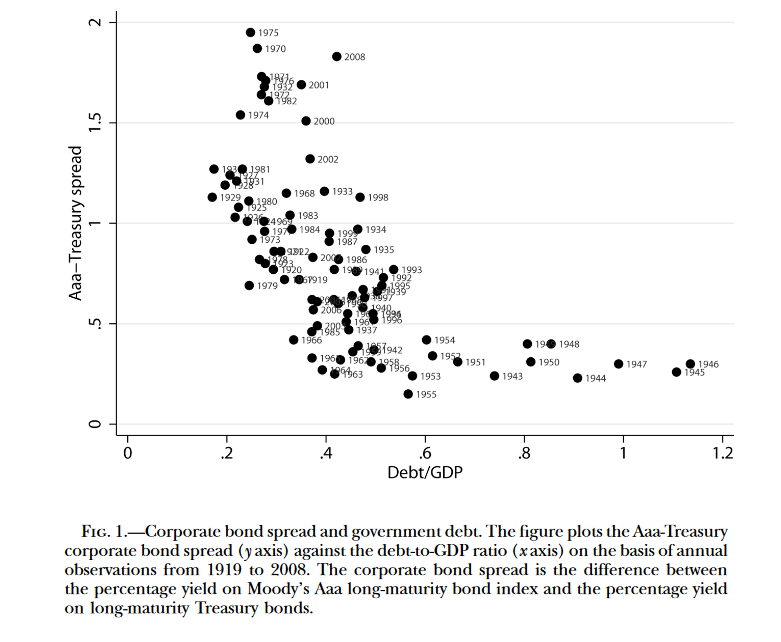
\includegraphics[width=0.7\textwidth]{krishna.png}
        \caption{Source: Krishnamurthy and Vissing-Jorgensen (2012)}
    \end{figure}
   \end{frame}

   \begin{frame}{Fiscal capacity}
    \begin{itemize}
        \item We need to modify the IGBC to account for the convenience yield.
            \begin{align*}
                B_t = \E_t \sum_{j=1}^\infty M_{t,t+j} \bp{T_{t+j}-G_{t+j}} + \E_t \sum_{j=1}^\infty M_{t,t+j} B_{t+j} \bp{\alb{1-e^{-\delta_{t+j}}}} 
        \end{align*}
        \item The new term $K_{t+j} \coloneq  B_{t+j} \bp{1-e^{-\delta_{t+j}}}$ represents the seignorage revenue from issuing debt.
        \item 
    \end{itemize}
   \end{frame}


   \begin{frame}{Fiscal capacity}
    \begin{itemize}
        \item Return to the example with $\beta_T = \beta_G = \beta_Y = 1$, but consider convenience yields. 
        \item Previously we said that the risk-free rate is equal to interest rate on treasuries, 1.5\%.
        \item If the convenience yield is 0.73\%, the true risk-free rate is higher -- 2.23\%.
        \item The PDV of surpluses is \begin{align*}
             \frac{0.25 - 0.225}{0.0523 - 0.02}=77\% \text{ of GDP}.
        \end{align*}
        \item The PDV of seignorage will depend on $\beta_K$ and the convenience yield.
        \item Set the convenience yield to 0.73\%. 
    \end{itemize}
   \end{frame}

   \begin{frame}{Fiscal capacity}
    \begin{itemize}
        \item If $\beta_K=1$ (seignorage varies proportionally with GDP), then $r_K = 0.523$ and the PDV of seignorage is \begin{align*}
            \frac{0.0073}{0.0523 - 0.02}=23\% \text{ of GDP}.
       \end{align*}
        \item This means that fiscal capacity is $100\%$ of GDP.
        \item Two \al{counteracting} forces: 
        \begin{enumerate}
            \item Convenience yield generates seignorage.
            \item For a given interest rate, convenience yield means that the true risk-free rate is higher -- this lowers the fiscal capacity.
        \end{enumerate}
        \item Extra surplus increases fiscal capacity by \al{less} than without the convenience yield.
    \end{itemize}
   \end{frame}   

   \begin{frame}{Fiscal capacity}
    \begin{itemize}
        \item Most likely $\beta_K < 1$. 
        \item In the short run, convenience yields can be counter-cyclical (\alb{flight to safety}).
        \item This increases the seignorage term, without affecting the risk-free rate.
        \item Lowering $\beta_K$ to 0.584, increases fiscal capacity to 114\% of GDP.
    \end{itemize}
   \end{frame}   
  
 

   \begin{frame}{Fiscal capacity}
    \begin{itemize}
        \item Jiang et al. use two approaches to estimate the fiscal capacity of the US. 
        \item In the first approach they Congressional Budget Office (CBO) projections of tax revenue and non-interest spending for the next 31 years (2022-2052).
        \item CBO also forecasts interest rates and GDP.
        \item At the end of the projection horizon debt to GDP is 185\%.
    \end{itemize}
   \end{frame}   

   \begin{frame}{Fiscal capacity}
    \begin{itemize}
        \item Given $r^f = 1.5\%$, the risk premium on GDP to 3\% and the average growth rate 2\%, annual surpluses would have to be 4.625\% of GDP since 2052 to sustain debt to GDP of 185\%.
        \item The present value of that is 35.2 trillion.
        \item The present value of the surpluses between 2022 and 2052 is -21.1 trillion (negative).
        \item The fiscal capacity in 2022 is 35.2-21.1 trillion = 14.1 trillion.
        \item This is 8.2 trillion \al{below} the 22.3 trillion in debt outstanding at the end of 2021.
    \end{itemize}
   \end{frame}  

   \begin{frame}{Fiscal capacity}
    \begin{itemize}
        \item This is already a generous estimate of the fiscal capacity.
        \item It assumes that the government can start running surpluses in 2052.
        \item It assumes acyclicality of taxes and spending.
        \item Another problem: duration mismatch.
        \item Surpluses are far in the future, fiscal capacity sensitive to small changes in the risk-free rate. 
    \end{itemize}
   \end{frame}    

   \begin{frame}{Fiscal capacity}
    \begin{itemize}
        \item The second approach: create forecast of cash flows using a VAR model.
        \item The model captures the cyclicality of tax and spending ratios.
        \item It captures multiple aggregate sources of risk:       inflation, interest rates, the price-to-dividend ra-
        tio in the stock market, and shocks to tax and spending rates.
        \item They calculate total fiscal capacity in two ways: (a) assume the discount rates are the same for taxes and spending, (b) model the SDF. 
    \end{itemize}
   \end{frame}  


   \begin{frame}{Fiscal capacity}
    \begin{figure}
        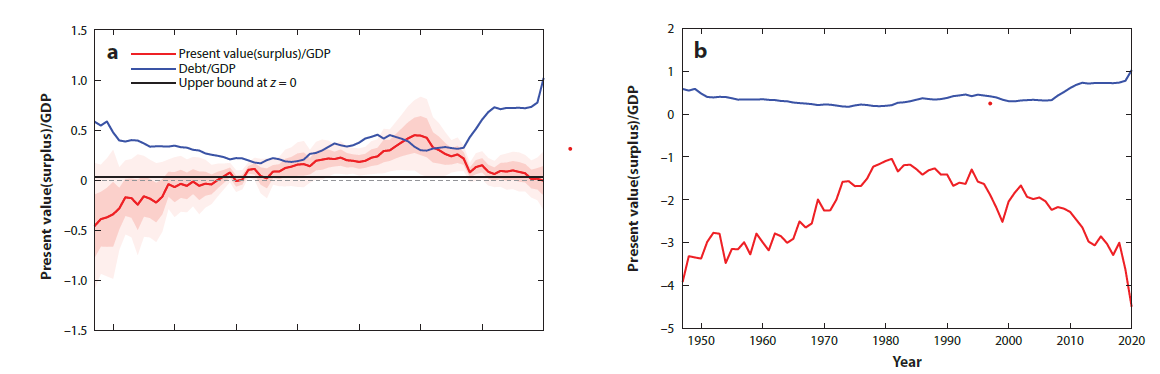
\includegraphics[width=1\textwidth]{capacity2.png}
        \caption{Source: Jiang et al. (2023)}
    \end{figure}
   \end{frame}


   \begin{frame}{Bond valuation puzzle}
    \begin{itemize}
        \item These estimates suggest a much lower fiscal capacity than the market value of outstanding debt.
        \item Possible explanations: \begin{itemize}
            \item Convenience yields?
            \item Bubble?
            \item Global safe asset supplier?
            \item Mispricing?
            \item Fiscal correction?
            \item Large-scale asset purchases and financial repression?
    \end{itemize}
\end{itemize}
   \end{frame}

   \begin{frame}{Bond valuation puzzle}
    \begin{itemize}
        \item Similar calculations for other countries suggest that the US is an outlier.
        \item For example, for the UK after World War 2 fiscal capacity was 82\% of GDP, but the debt to GDP ratio was 53\%.
        \item It was different in 1729-1946 when fiscal capacity was 68\% of GDP, but the debt to GDP ratio was 87\%.
        \item Developing countries: procyclical surpluses, debt prices react strongly to funamentals (unlike the US).
    \end{itemize}
   \end{frame}   

\end{document}